%\documentclass[letterpaper,12pt]{article}
\documentclass[epsf]{article}
\usepackage{graphicx}
\usepackage{amsmath, amssymb, latexsym,hyperref} 
\usepackage{amsfonts}
\usepackage{array}
\usepackage{verbatim}
\usepackage{bm}
\usepackage{enumerate}
\usepackage[margin=1in]{geometry}

\hypersetup{
    bookmarks=true,          % show bookmarks bar?
    unicode=false,             % non-Latin characters in Acrobat�s bookmarks
    pdftoolbar=true,           % show Acrobat�s toolbar?
    pdfmenubar=true,        % show Acrobat�s menu?
    pdffitwindow=false,      % window fit to page when opened
    pdfstartview={FitH},     % fits the width of the page to the window
    pdftitle={My title},         % title
    pdfauthor={Author},     % author
    pdfsubject={Subject},   % subject of the document
    pdfcreator={Creator},   % creator of the document
    pdfproducer={Producer}, % producer of the document
    pdfkeywords={keyword1, key2, key3}, % list of keywords
    pdfnewwindow=true,      % links in new PDF window
    colorlinks=true,               % false: boxed links; true: colored links
    linkcolor=red,                  % color of internal links (change box color with linkbordercolor)
    citecolor=green,             % color of links to bibliography
    filecolor=magenta,         % color of file links
    urlcolor=cyan                % color of external links
}


\newcommand{\ds}{\displaystyle}
\newcommand\numberthis{\addtocounter{equation}{1}\tag{\theequation}}
\newcommand{\tthe}{\tilde\theta}
\newcommand{\tphi}{\tilde\phi}
\newcommand{\talph}{\tilde\alpha}
\newcommand{\te}{\tilde e}
\newcommand{\ta}{\tilde a }
\newcommand{\ti}{\tilde i}
\newcommand{\tw}{\tilde \omega}
\newcommand{\tW}{\tilde \Omega}
\newcommand{\tM}{\tilde M}
\newcommand{\tn}{\tilde n}

\font\twelverm=cmr12
\font\twelvebf=cmbx12
\font\tenbf=cmbx10
\font\tenrm=cmr10
\font\tenit=cmti10
\font\elevenbf=cmbx10 scaled\magstep 1
\font\elevenrm=cmr10 scaled\magstep 1
\font\elevenit=cmti10 scaled\magstep 1
\font\ninebf=cmbx9
\font\ninerm=cmr9
\font\nineit=cmti9
\font\eightbf=cmbx8
\font\eightrm=cmr8
\font\eightit=cmti8
\font\sevenrm=cmr7

%
\textwidth = 7.0truein
%\textheight = 8.5truein
\oddsidemargin=-0.2truein
\evensidemargin=-0.2truein
\topmargin=0.0truein
%\notename{UCD/IIRPA} \notenumber{92-24}

\begin{document}

\begin{center}{{\twelvebf Notes on the Kepler Fitting Method}}
		\vglue 0.5cm
 	       {\tenrm JOHN R.\,\,SMITH\\}
	       {email: john.smith7@ngc.com\\}
		\vglue 0.25cm
%	        \baselineskip=13pt
	       {\tenit Northrop-Grumman Corporation\\
	       301 Voyager Way\\}
                \baselineskip=12pt
                 {\tenit Huntsville, Alabama USA\\}
		\vglue 0.5cm
                 {\rm December 3, 2020\\}
\end{center}
\section{Orbit Determination using Kepler Elements}

The object of this project is to develop an Orbit Determination (OD) method based on using Kepler Elements as State Vectors.\\

As regards possible motivations for using such state vectors, consider the standard Cartesian State Vectors and the methods used to represent the trajectory. Basically the standard approach considers the actual trajectory to be a kind of stochastic process where discrete observations are used to update the state vector. If such an approach was imagined to be taken to the limit of continuous updating, then it is very likely that the trajectory would become a stochastic process similar to Brownian motion except that the mean time dependence would be given by the assumed motion model. There is a fundamental mathematical problem which may be of concern for this approach and that is that even continuous stochastic processes such as Brownian motion are continuous but nowhere differentiable. Brownian motion can be considered as the ``integral'' of white noise and there is a method of mean-squared integration that yields the reverse -- that the mean-square ``derivative'' of Brownian motion is white noise. Therefore one wonders what significance the time-rate-of-change estimates that come out of updating a State Vector really are, or if there are fundamental limitations intrinsic to the method. Similar problems exist in the subject of polymer physics based on path-integral methods -- usually a "stiffness" term is inserted ad-hoc into the mathematics to insure some kind of limits on the fluctuations which are encountered in numerical work. Such stiffness terms in a polymer are similar to demanding some level of ``smoothness'' in addition to continuity. So too with orbit determination methods. Are there intrinsic limitations on the velocity determination which are due to the state vector update methods? The idea behind this study is to examine replacing Cartesian elements with a quasi-state state vector in terms of Kepler elements and adopt a parameter estimation approach which represents not only the trajectory but also all the time-derivatives of that trajectory in a smooth manner and see if the resulting fit has a better performance vis-a-vis the covariance structure in position as well as velocity space.\\

The data can be a combination of measurement variables including: position $\vec{r}$, velocity $\vec{v}$, range $\rho$, line-of-sight unit vectors (angles $\theta$ and $\phi$ -- or Az and El), range-rate $\dot\rho$, and angular rates $\dot\theta$ and $\dot\phi$ or any other quantity that can be expressed in terms of the osculating classical Kepler elements and time. We will start off by using only line-of-sight directions as the measurement data and assume that we are provided with line-of-sight unit vectors as measured by a moving observer -- which is not necessarily fixed on the surface of the earth. The unit vectors are assumed to be given in the Earth-Centered Inertial (ECI) frame and are determined by 2 angles which can be taken as Az and El or as $\theta$ and $\phi$ in spherical polar coordinates as measured in the ECI-referential frame attached to the sensor location (the coordinate system whose unit vectors are parallel to the ECI system, but carried along by the sensor). In this case the dimension of the measurement data is 2 corresponding to the angular information. But we will allow for more measurement flavors and multiple sensors. \\

One way to model the problem of OD is to find a method of predicting the time dependence of the angular variables represented as a column vector $\alpha(t_i) = [\theta(t), \phi(t)]$ for the line-of-sight in such a way to minimize the statistical measure $\chi^2$ defined by 
\begin{align*}\chi^2 = {1\over2}\sum_{i=1}^N\, [\alpha(t_i) - \talph_i]^T \hbox{Cov}_i^{-1}[\alpha(t_i) - \talph_i],\numberthis\label{eqnChiSq}\end{align*}where the sum is over the set of $N$ measurements $\talph_i = [\tthe_i, \tphi_i], t = 1,2\hdots, N$ and we use brackets $[ ~~ ]$ to denote column vectors denote transposition of a vector or a matrix by $[~~ ]^T$.This method leads to the usual batch Least Squares Estimate (LSE) approach and can be generalized to include other variables such as range, range-rate and the others mentioned in the list above by extending the vectors to dimension $n$ and the covariance structure to an $n$-by-$n$ real symmetric matrix.  The rank $n$ of Cov for each term on the Right Hand Side (RHS) of the above sum and the number of independent measurements in the data which are required in order to make an estimate of the full set of parameters. Typically the number of measured variables is less than the number of parameters being determined and therefore a minimum number of independent measurements are required before the problem reaches full rank and a estimate of the set of parameters possible. Of course, if an initial estimate of the state is available, then of course, updates to the parameter values can ensue via a sequential revision of the Least Squares method. \\

As an example, an extension of this problem to the list of variables mentioned at the beginning would require a measurement vector of the form 
$$\alpha = [\vec{r}, \vec{v}, \rho, \theta, \phi, \dot\rho, \dot\theta, \dot\phi]$$ at time $t$ and a corresponding prediction vector of the same quantities given in terms of the Kepler elements and the time $t$. This will be apparent to us as we proceed as the estimation process will involve solving a linear system and that linear system is constructed from a sum of terms each of which may have less rank than the set of parameters requires, but enough independent measurements are used so that the complete linear system has full rank. Otherwise the problem in batch mode is unsolvable -- we need to have enough data to perform the estimate from scratch. This will not preclude incorporating new data with less than full rank to an initial estimate. \\

It doesn't hurt to work out a general procedure for handling many flavors of measurements and then apply it to lower dimensional problems by simply turning off some of the terms -- a procedure that can do more, can also do less. We will apply this problem to the case of line-of-sight measurements, by ignoring the irrelevant terms in the vector of observations.\\

Other method of approaching the OD problem might use the Minimum Variance Estimate (MVE), or Maximum Likelihood (ML), or Restricted Maximum Likelihood (REML). We will work out a method based in minimizing $\chi^2$ which has ML as its counterpart, MVE and REML are analogous. In REML the object is to minimize the ``error contrasts'' which is similar to minimizing the variances occurring in the problem.\\

The next thing to notice is that the minimization of $\chi^2$ has several manifestations. One can attempt to minimize $\chi^2$ by computing its derivatives with respect to the parameter set 
$Z = [z_1, z_2, z_3, \hdots , zm]$ by computing the derivative vector and solving for 
\begin{align*}{\partial \chi^2\over \partial z_j} = 0,~~j = 1,2,\hdots m \numberthis \label{eqnFirstOrder}\end{align*}
This method usually is based on a first order Taylor expansion of the prediction vector $[\theta(t), \phi(t)]$ in terms of the parameter set $Z$ and, in the case of nonlinear functions, performing iterations via the Newton-Raphson technique. 
Application of the first order technique can be found in \cite{Avery} to vertex fitting methods in High Energy Physics which are the underlying theory for the SCOUT methods\cite{SQUAW}\\

This isn't the only way of setting up the minimization problem. For example one can look at the problem from the point of view of finding the critical points of the gradient of $\chi^2$ itself without worrying first about whether $\chi^2$ is a minimum. In other words, there is a second order method which seeks to solve for the critical points by expanding the gradient in its own linear Taylor expansion, viz., 
$${\partial \chi^2\over \partial z_j} \approx {\partial \chi^2\over \partial z_j} \biggl|_{\hat{Z}} + \sum_{k=1}^N  {\partial^2 \chi^2\over \partial z_j \partial z_k} \biggl|_{\hat{Z}}\,\delta z_k,\quad j =1,2,\hdots, m,$$
where $\delta z_k = z_k - \hat{z}_k$ and $\hat{Z}$ is the expansion point for the Taylor series.  In this method the idea is to apply Newton-Raphson iteration to the equation 
$$0 = {\partial \chi^2\over \partial z_j} \biggl|_{\hat{Z}} + \sum_{k=1}^N  {\partial^2 \chi^2\over \partial z_j \partial z_k} \biggl|_{\hat{Z}}\,\delta z_k,\quad j =1,2,\hdots, m,$$which can be turned into a linear system to solve for the increment $\delta z_k$ to be used as the expansion point $$\hat{Z} \rightarrow \hat{Z} + \delta z$$to be used in the next iteration. This updating is continued via Newton-Raphson iteration until (hopefully) the method converges and $\delta Z \rightarrow \bf{0}$ (the zero vector). The second order method takes more information into account, for example it uses the information on how the derivatives of $\chi^2$ themselves are changing as a function of the parameter set. Therefore this method also requires computing the Hessian matrix, $\bf H$, whose components are given by
$$H_{ij} = {\partial^2 \chi^2\over \partial z_j \partial z_k}, \quad i,j = 1,2,\hdots m$$

We will proceed to outline both the first order method as well as the second order method with respect to the prediction vector for the line-of-sight prediction vector $[\theta(t), \phi(t)]$. To apply the first order method we make the assumption that the linear approximation to the prediction vector near the minimum of $\chi^2$ is ``good enough'' meaning that is is ``reasonably linear'' where the minimum of $\chi^2$ is located. The may not be the case especially if the parameter space has hard boundaries and the minimum is located near those boundaries -- various problems can occur, e.g, the parameters may become complex numbers due to exceeding the physical range of possibilities.\\


\input{"BFGS Method.tex"}
\input{"FundamentalOrbitDetermination.tex"}
\input{"Sequential.tex"}
\section{Application of the first order method}
Let us denote the prediction vector as 
$${\alpha(t)} = 
\begin{bmatrix}
\theta(t) \\
\phi(t)\\
\end{bmatrix}\hbox{ and the measurement data vectors as  } 
\tilde\alpha = 
\begin{bmatrix}
\tilde\theta\\
\tilde\phi\\
\end{bmatrix}$$In this case the dimension $n$ of the measurement vector is $n=2$. We expand $\alpha(t)$ about a suitably chosen expansion point (which will be iterated) in the $m$ parameters
$Z_A$, and define $\alpha(t)|_{Z_A} \equiv \alpha_A(t)$ as the value of the predicted observation at time $t$ with respect to the current parameter set (the expansion point $A$). We also define the 
differences $\delta\alpha(t) = \alpha(t) - \alpha_A$ and $\delta\tilde\alpha(t) = \tilde\alpha - \alpha_A$.\\

The first order method involves a Taylor expansion of the prediction functions $\alpha_i(t)$ in terms of the components of the basic parameter set $\bf Z$:

$$\alpha(t) \approx \alpha+A(t) + {\partial \alpha(t)\over \partial Z_k}\big|_{Z_A}\, \delta z_k$$In order to economize the notation let us define the following $n$-by-$m$ Jacobian matrix $\bf D$:
$$D_{ik}={\partial \alpha_i(t)\over \partial Z_k}\big|_{Z_A}, \quad i=1,2,\hdots,n\quad k = 1,2,\hdots m$$

Performing the differentiation of each term in the sum on the RHS of Eq.\eqref{eqnChiSq}, each of the $i=1,2\hdots,N$ measurements yields a set of equations of the form
$${\bf D}(t_i)^T\hbox{\bf Cov}^{-1} {\bf \delta \tilde\alpha}(t_i) = {\bf D}(t_i)^T\hbox{\bf Cov}_i^{-1} {\bf D}(t_i)\delta {\bf z}$$summing over the $N$ data points we obtain the LSE equation which the increment
$\bf \delta z$ must satisfy
$${\bf \delta z} = \bigg[\sum_{i=1}^N {\bf D}(t_i)^T\hbox{\bf Cov}_i^{-1} {\bf D}(t_i) \bigg]^{-1} \bigg[ \sum_{i=1}^N {\bf D}(t_i)^T\hbox{\bf Cov}^{-1} {\bf \delta \tilde\alpha}(t_i) \bigg]$$

At this point in the development please not that the rank of each of the terms of the form ${\bf D}(t_i)^T\hbox{\bf Cov}_i^{-1} {\bf D}(t_i)$ is at most of $\hbox{rank({\bf Cov})}$. The Jacobian terms usually
don't lower the rank as long as the transformation they correspond to at 1-to-1. Therefore if $\hbox{rank({\bf Cov})} < \hbox{ length of } {\bf \delta z}$, then it is necessary to obtain enough data such that
the sum over the data is full rank and the linear system has a unique solution. \\

The above LSE estimate can also be sequentialized to emulate a Kalman filter method. As is usually the case, the convergence properties of iterative fitting methods such as the
first or second order fitting methods depend on the closeness of the initial estimate of the parameters and the goodness of the assumption of linearity used in the Taylor expansion. The Angles-Only
orbit determination method involves many transformations and opportunities to test out these assumptions.
\section{Application of the second order method}

The second order method involves taking the first and second derivatives of Eq.\eqref{eqnChiSq} which we write for a general vector of observations and predictions as:

\begin{align*}\chi^2 = {1\over2}\sum_{i=1}^N\, [\alpha(t_i) - \talph_i]^T \hbox{Cov}_i^{-1}[\alpha(t_i) - \talph_i]\end{align*}

Under the assumption that the covariance matrices are symmetric we can compute the first derivative as
$${\partial \chi^2\over \partial z_j}  = \sum_{i=1}^N\, \bigg[{\partial\alpha(t_i)\over\partial z_j}\bigg]^T \hbox{Cov}_i^{-1}[\alpha(t_i) - \talph_i] \quad j =1,2,\hdots, m,$$

Proceeding to the second derivatives of Eq.\eqref{eqnChiSq} we obtain:
$${\partial^2 \chi^2\over \partial z_j\partial z_k}  = 
\sum_{i=1}^N\, \bigg[{\partial^2\alpha(t_i)\over\partial z_j\partial z_k}\bigg]^T \hbox{Cov}_i^{-1}[\alpha(t_i) - \talph_i]  + \bigg[{\partial\alpha(t_i)\over\partial z_j}\bigg]^T \hbox{Cov}_i^{-1}\bigg[{\partial\alpha(t_i)\over\partial z_j}\bigg]
\quad j,k  =1,2,\hdots, m.$$

We define the Jacobian matrix, $\bf J$ corresponding to the partial derivatives appearing by 
$$J_{ij} = \bigg[{\partial\alpha(t_i)\over\partial z_j}\bigg]$$and the Hessian matrix, $\bf H$, of mixed partial derivatives as 
$$H_{jk}(t_i) = {\partial^2\alpha(t_i)\over\partial z_j\partial z_k}$$

With $\bf J$ and $\bf H$ defined in this manner the first and second derivatives can be written as 
$${\partial \chi^2\over \partial z_j}  = \sum_{i=1}^N\, J_{ji}^T \hbox{Cov}_i^{-1}[\alpha(t_i) - \talph_i] \quad j =1,2,\hdots, m,$$

and 

$${\partial^2 \chi^2\over \partial z_j\partial z_k}  = 
\sum_{i=1}^N\, \bigg[H_{jk}(t_i)^T \hbox{Cov}_i^{-1}[\alpha(t_i) - \talph_i]  + J_{ji}^T \hbox{Cov}_i^{-1}J_{ik} \bigg] \quad j,k  =1,2,\hdots, m.$$

The idea of the second order method is to expand the gradient of $\chi^2$ into a Taylor series and set the resulting components each to 0 and apply Newton-Raphson iterations to the result as follows: 
$${\partial \chi^2\over \partial z_j} \approx {\partial \chi^2\over \partial z_j} \biggl|_{\hat{Z}} + \sum_{k=1}^N  {\partial^2 \chi^2\over \partial z_j \partial z_k} \biggl|_{\hat{Z}}\,\delta z_k = 0,\quad j =1,2,\hdots, m,$$
which leads a linear system for the increment vector $\delta z_k$
$$\delta z_k =  -\sum_{j=1}^m\bigg[\sum_{i=1}^N\, \big[H_{jk}(t_i)^T \hbox{Cov}_i^{-1}[\alpha(t_i) - \talph_i]  + J_{ji}^T \hbox{Cov}_i^{-1}J_{ik} \big] \bigg]^{-1} \bigg[ \sum_{i=1}^N\, J_{ji}^T \hbox{Cov}_i^{-1}[\alpha(t_i) - \talph_i]  \biggl|_{\hat{Z}}\bigg]$$

The above system can be interpreted using matrix multiplication. Let $\bf V$ be the vector in the parameter space with components
$$V_j = \sum_{i=1}^N\, J_{ji}^T \hbox{Cov}_i^{-1}[\alpha(t_i) - \talph_i] $$ and $\bf M$ the matrix in the parameter space with components
$$M_{jk} = \sum_{i=1}^N\, \bigg[H_{jk}(t_i)^T \hbox{Cov}_i^{-1}[\alpha(t_i) - \talph_i]  + J_{ji}^T \hbox{Cov}_i^{-1}J_{ik} \bigg],$$
Then the solution to the linear system can be written in matrix form as
$${\bf \delta z} = - {\bf M}^{-1}{\bf V}$$



\section{Computation of the Predictions}

Assume the data consists of line-of-sight measurements from an observer whose position as a function of time is $\vec{R}_{obs}(t)$. At each of the measurement times $t_i$, the observer is located at $\vec{R}_i = \vec{R}_{obs}(t_i)$ and makes a measurement of a line-of-sight vector ${\bf l}_i = [x_i, y_i, z_i]$ which we assume has been transformed into the Earth-Centered Intertial (ECI) reference system by a suitable transformation from whatever reference frame the measurement was taken in Earth-Centered Earth Fixed (ECEF) or some other typical observation frame. Assuming we have an initial estimate of the object-of-interest's state vector at a reference time $t_0$ which might be given in position and velocity space or the classical orbital elements or others. We can implement the respective equations of motion to propagate these state vectors as needed to the current time of interest. Obviously whatever state vectors are used as the underlying independent variables, to compute the predicted state which can be compared to the observed data, we must identify the functional form this prediction is to take. As an example, the predicted line-of-sight vector is 
$$\vec{l}_i = \vec{R}(t_i) - \vec{R}_i$$
One can translate this vector into more convenient quantities related to the data format e.g., if the range is not measured, then we can work with $(Az, El)$ or $\theta, \phi$. In terms of spherical polar coordinates this vector's components in ECI are given by 
$$\vec{l} = [l_x, l_y, l_z] = l_{\hbox{mag}} [\sin(\theta)\cos(\phi), \sin(\theta)\sin(\phi), \cos(\theta)],$$where $\l_{\hbox{mag}} = \sqrt{l_x^2 + l_y^2 + l_z^2}$. The unit vector that describes the line-of-sight direction, is given by 
$$\vec{u} = [\sin(\theta)\cos(\phi), \sin(\theta)\sin(\phi), \cos(\theta)]$$and the relationship between these quantities and the components of $\vec{l}$ are given by
\begin{align*}
l_{\hbox{mag}} &= \sqrt{l_x^2 + l_y^2 + l_z^2}\\
\theta               &= \cos^{-1}(l_z/l_{\hbox{mag}})\\
\phi                  &= \hbox{atan2}(l_y,l_x)\\ \numberthis \label{eqnLOS}
\end{align*}Note that atan2$(l_y,l_x)$ takes care of the quadrant determination automatically. If the range rate and rates of change in the angles were available, we could make room for those measurements as well in the above list. Some care may still be needed so that directions near $\phi=0$ and $\phi=2\pi$ are taken to be close to each other and not far apart. Closeness in phi can be determined by using dot products and cross products followed by a further atan2 to pin down the actual relative phi-angle difference in such cases. \\

Ultimately we need to work out the Jacobians that will take us all the way back to the propagated state vectors in such a manner that the LSE method can be iterated and the state vector estimate updated. We shall proceed starting with the items corresponding to the above list and work our way back to the relevant state vector by either application of the chain rule, or by direct computation based on the method of backwards differentiation which determines each Jacobian based directly on the functional dependence according to the respective composition of the functions involved and their direct differentiation.
\section{Time Development of the Kepler Elements and Perturbation Theory}

The State Space approach in the time domain applied to sequential filtering methods is a standard approach. Control Theory and Stochastic Estimation still make use of the State Space model -- although there are other alternative approaches currently under development in Control Theory. \\

Some applications involve ordinary differential equations which might represent some sort of ``propagation'' in time or perhaps some other independent variable. These differential equations are very often non-linear in the dependent variables and normally one resorts to a linearization method so that standard State-Space methods can be employed -- although this needs to be implemented iteratively in the hopes that the initial estimates are ``good enough'' and that the 
iteration process converges to the correct solution (if it converges at all).\\

Let us apply these concepts to the OD problem. The standard State Space representation is in terms of position, velocity and time. The relevant state then incorporates position and velocity which then are envisioned as functions of the independent variable (time). 

The typical State Vector, $Y(t)$, representation for the OD problem is therefore of the form 
$$Y(t) = 
\begin{bmatrix}
\vec{r}(t)\\
\vec{v}(t)\\
\end{bmatrix}$$and then the equations of motion can be written as a first order system of differential equations for the time development in the following form:
$$\dot Y(t) = 
\begin{bmatrix}
\vec{\dot r}(t)\\
\vec{\dot v}(t)\\
\end{bmatrix} =
\begin{bmatrix}
\vec{v}(t)\\
\vec{\ddot r}(t)\\
\end{bmatrix}
$$

At this point, one usually substitutes for $\vec{\ddot r}$ based on Newton's 2nd Law (assuming constant mass) $$\vec{F} = m\vec{\ddot r}$$where $m$ is the mass and $\vec{F}$ are the forces acting on the mass. Newton's 2nd Law can also be extended to non-inertial coordinate systems in the usual manner provided care is taken to adjust the mass terms and forces accordingly. These adjustments are standard in OD theory where the reference origin is the center of the earth
and the position vector is given by relative position between the center of the earth and the sensor (wherever the sensor is located -- attached to the earth, or orbiting, etc.).\\

Another approach to representing the State Vector associated with an orbiting trajectory is to use the classical Kepler elements in the form
$$K(t) = [e(t), a(t), i(t), \omega(t), \Omega(t), M(t)]^T$$where $e$ is the eccentricity, $a$ is the semi-major axis, $i$ is the inclination, $\omega$ is the argument at periapsis, $\Omega$ is the longitude of the line of nodes, and $M$ is the mean anomaly and all of these elements
are given at time $t$. In the case of the pure Kepler orbit, then these classical elements are all constant except for the mean anomaly which is a linear function of time. 

To apply the state space approach to the OD estimation problem in the presence of perturbations one normally linearizes the equations of motion by expanding them about a reference orbit which is chosen to approximate the true orbit of interest closely but a the same time to have a simpler time development because the perturbations are left out of the time evolution of the reference orbit. This method goes by the name of ``chief and deputy'' where the chief is the reference 
orbit and the deputy is the orbit of interest. One works with the relative difference between the chief and deputy. Of course, to get back to the deputy's orbit with respect to the earth, then the components of the chief are added to the deputy by vector addition. Because a pure Kepler orbit (pure $1/r^2$ gravity with no perturbations) has a simple time development, it can be used as the chief and the time development involves numerically solving Kepler's equation. Even with a numerical solution of Kepler's equation in hand, all the subsequently required derivatives present no problem due to application of the Implicit Function Theorem to Kepler's equations: $M = E - e\sin(E)$ (with E,M,e known numerically). \\

Regarding the gravitational model, we will work with up-to-J6 zonal harmonics and consider the pros-and-cons of various methods of expanding the equations of motion about a Kepler orbit used as the reference as a relative origin. 
The up-to-J6 zonal harmonics leads to a gravitational potential of the form
\begin{align*}
\Phi = {mu\over r}\big[ 1  &+ {J_2\over2r^2}(1-3\sin^2\delta ) \\
                                        &+ {J_3\over2r^3}(3-5\sin^2\delta )\sin\delta\\
                                        &+ {J_4\over8r^4}(3-30\sin^2\delta +35\sin^4\delta)\\
                                        &+ {J_5\over8r^5}(15-70\sin^2\delta) +63\sin^4\delta)\sin\delta\\
                                        &+ {J_6\over16r^6}(5-105\sin^2\delta +315\sin^4 - 231\sin^6\delta)\\
                                        &+ \epsilon]\\ 
\numberthis \label{eqnPhi}
\end{align*}where $\mu$ is the graviational constant, $J_i$ us the coefficient of the $i$th zonal harmonic, $\epsilon$ represents terms of higher order and other missing harmonics (tesseral and sectoral).  The distance from the center of
the earth is measured in canonical units is $r$ and $\sin\delta = z/r$ where $z$ is the respective coordinate along the North-South axis in the same units as $r$. If canonical units are not used, then replace $r$ by $r/a_e$, where $a_e$ is the equatorial radius of the earth. \\

In the case of the spherical and homogenous earth, the gravitational potential is just 
$$V = {\mu\over r}$$which gives rise to the pure Kepler orbits where the classical elements $e,a,i,\omega,\Omega$ are constants and $M$ is a linear function of time such that $M=0$ at periapsis. The mean anomaly for this case is given by 
$M = n(t-t_p)$ and $n$ is the mean motion, $t$ is the time, and $t_p$ is the clock time at periapsis. The disturbing potential $R$ due to the gravitational perturbations beyond the purely spherical earth is defined as 
$$R = \Phi - V$$

Some approaches to approximating the equations of motion make use of binomial expansions and trigonometric series. I believe the most expedient approach is to use Taylor expansions of the full expressions so that the linear term is determined without recombining the binomial and trigonometric series into first order and second order terms. Also implicit differentiation eliminates application of similar expansions of Kepler's equation -- so why not try to work with Taylor expansions throughout since only the linear terms are kept in the expansion of the deputy's orbit relative to the chief? Another thing to note is that position and velocity states are rapidly varying and perhaps it is better to describe the trajectory in a representation that is less rapidly varying.
On the other hand, perturbations tend to remain small in the position and velocity space representation which might have advantages over other representations where possible singularities might be present in the expansion of the equations of motion. \\


\section{Linearization of the Perturbed Equations of Motion in Position and Velocity Space}

Since perturbations are supposed to be ``small effects'' one approach to linearizing the equations of motion in terms of the Kepler elements it to work out the corresponding effects in
position and velocity space and then transform the results over to Kepler space by implementing the appropriate Jacobians. 

Since we need to expand the equations of motion about the Kepler chief's orbit we will first examine the situation based on relative position and velocity state vectors and see how they can be transformed over to Kepler classical elements.
The the disturbing potential is given by $R$ from above. Now the forces which arise from the contribution of $R$ follow in the usual manner by taking gradients:
$$\vec{F}_D = \nabla R$$Using the standard position and velocity state vector representation $Y(t)$ from above, we have for the equations of motion, the following linear system corresponding to the time rate of change of deputy's state vector as seen from the chief: 
$$\dot Y_{deputy}(t) = 
\begin{bmatrix}
\vec{\dot r}(t)\\
\vec{\dot v}(t)\\
\end{bmatrix} =
\begin{bmatrix}
\vec{v}(t)\\
\vec{\ddot r}(t)\\
\end{bmatrix} = 
\begin{bmatrix}
v_x\\
v_y\\
v_z\\
\nabla_x D\\
\nabla_y D\\
\nabla_z D\\
\end{bmatrix}
$$
The acceleration due to the $D$ is given by $\vec{a} = \nabla(D)$.
We can assume that the initial conditions for this problem are given by the following state vector where the deputy and chief are together at $t_0$:
$$Y_{deputy}(t_0) =  [0, 0, 0, \nabla_xD, \nabla_yD, \nabla_zD]^T$$

Assuming that small changes in coordinate space are related by Jacobians to small changes in Kepler space we might expect 
that the accelerations could be expanded about their values at $t_0$ in a Taylor series corresponding to small changes in coordinate space along the lines: 
$$a_i \approx a_i|_{\hat Z} + \sum_{j=1}^3{\partial a_i\over \partial Z_j}|_{\hat{Z}}(Z_j - \hat{Z}_j) 
= {\partial D\over\partial z_i}|_{\hat Z} + \sum_{j=1}^3{\partial^2 D\over \partial Z_i \partial Z_j}|_{\hat{Z}}(Z_j - \hat{Z}_j),$$
where the sum over $j$ corresponds to a sum over the spatial coordinates $Z_1 = x, Z_2 = y, Z_3 = z$. \\

If the accelerations are almost constants over a short time period then the velocity of the deputy with respect to the chief would go approximately like
$$\vec{v}(t) \approx \vec{a} \times (t-t_0)$$

Let $\bf H$ be the 3-by-3 matrix of second derivatives of the disturbing potential with respect to the spatial coordinates, i.e., 
$$H_{ij} = {\partial^2 D\over \partial Z_i \partial Z_j}, \quad i,j = 1,2,3$$

Inserting these approximations into the time rate of change of the relative coordinates of the deputy and chief we have approximately

$$\dot Y_{deputy}(t) \approx 
\begin{bmatrix}
{\vec v} - {\vec v}_K\\
{\bf \nabla} D\\
\end{bmatrix} \approx 
\begin{bmatrix}
{\bf 0}_3\\
{\bf \nabla} D\\
\end{bmatrix}_{\hat Z}  + 
\begin{bmatrix}
 0         &  {\bf I}_3\\
{\bf H}  &0\\
\end{bmatrix}_{\hat Z} 
\begin{bmatrix}
 \vec{r}- \vec{r}_K\\
\vec{v} - \vec{v}_K\\
\end{bmatrix} 
$$
The first term on the RHS represents the Inhomogeneous vector term, ${\bf I} = [{\vec v} - {\vec v}_K, {\bf \nabla} D]$, in the expanded equations of motion and the second term on the RHS is the Homogeneous matrix term $\bf Q$. The eigenvalues of the Homogeneous term determine the stability properties of the solution of the system of differential equations. If the eigenvalues have real parts which are $>1$ then the solution will grow unboundedly at $t$ increases. \\
\begin{figure}[hptp]
\begin{center}
   \resizebox{0.56\linewidth}{0.56\linewidth}{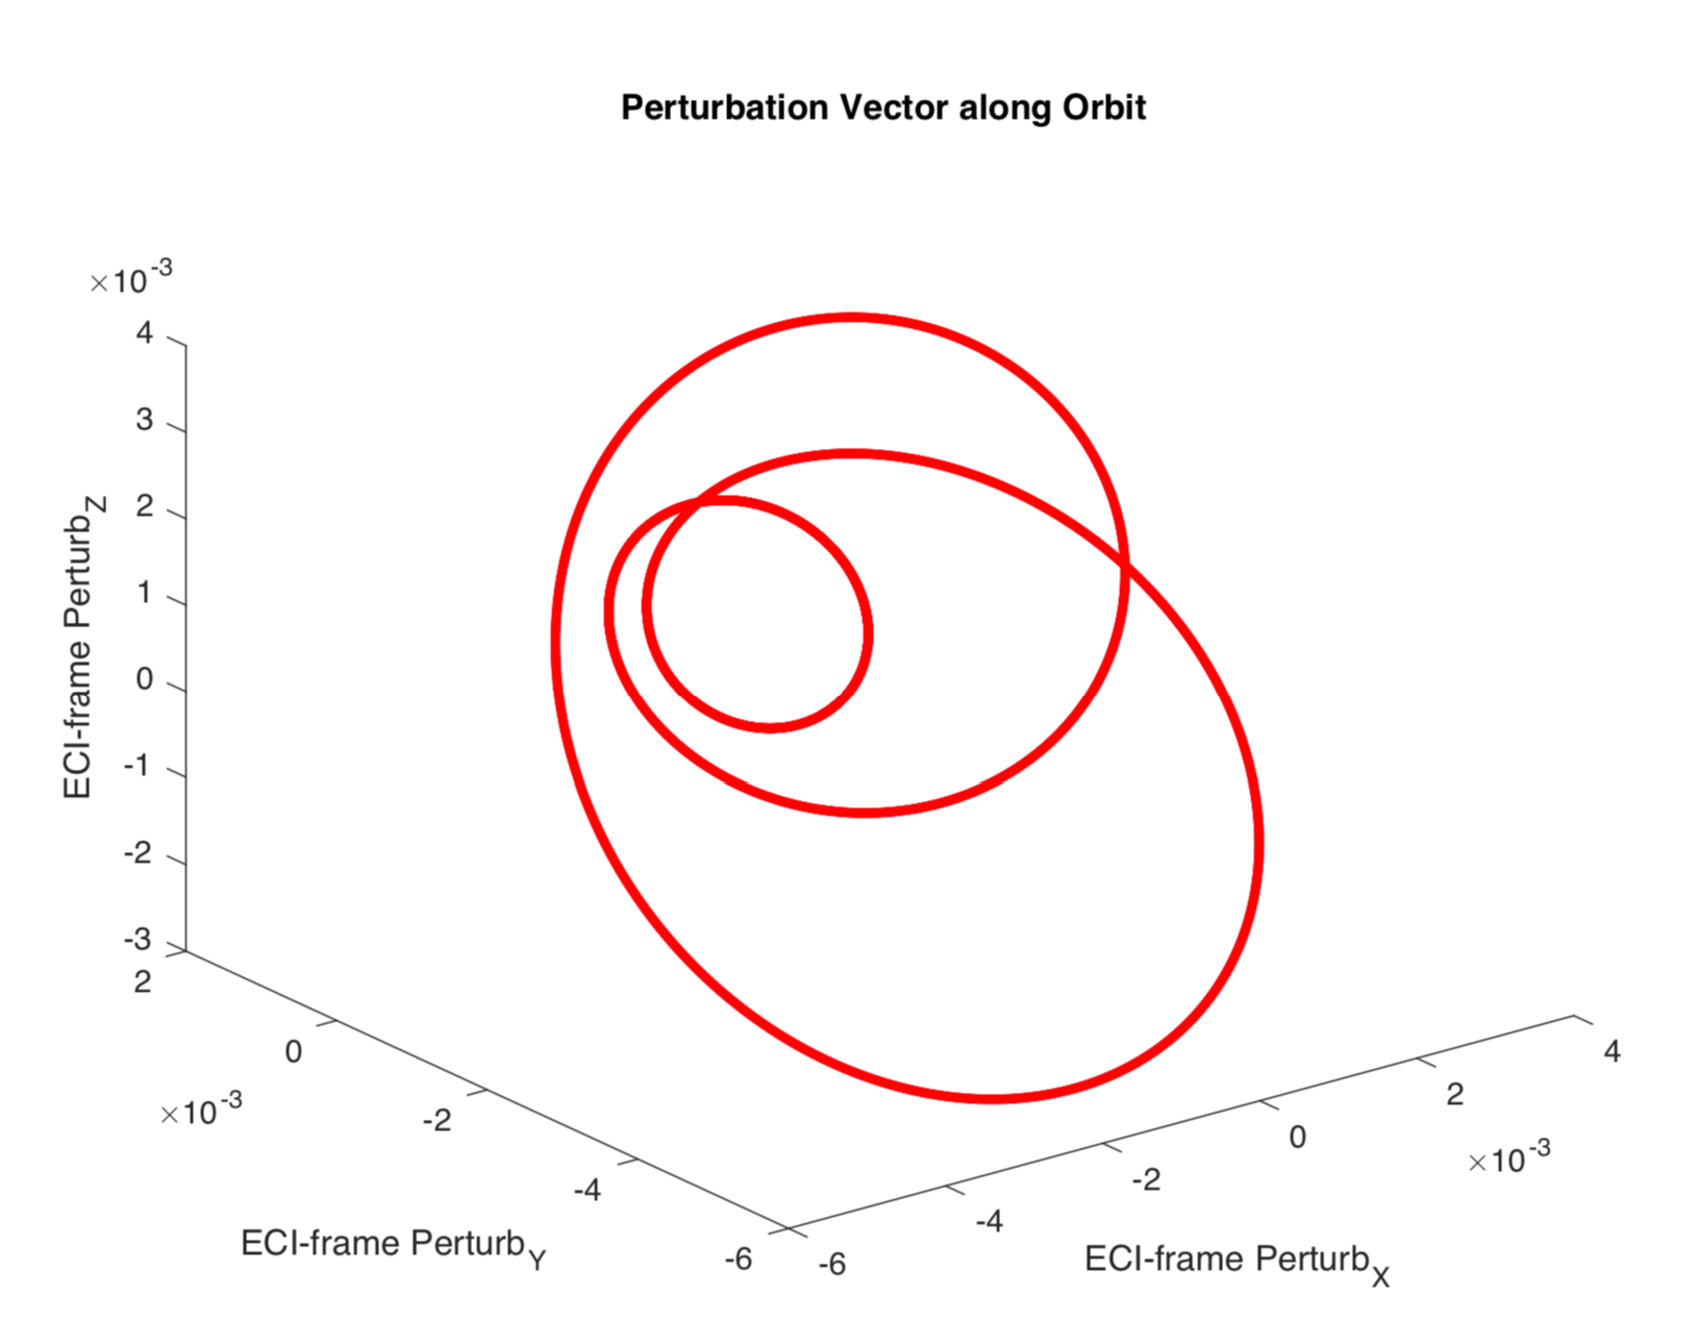
\includegraphics{EigenvaluesJ6.pdf}}
   \caption{J6 Perturbations vector transported around one orbit}
   \label{fig:J6Perturbations} 
\end{center}
\end{figure}

Given that we consider the differences between the components of the chief and the deputy to be small, the relative displacements in position and velocity space and in Kepler space should transform the way vectors transform under
change of coordinates:$$\overline{A}^j = \sum_{k=1}^m{\partial \overline{x}^j\over \partial x^k}A^k$$%with summation over the repeated index $k$ assumed by convention. 
Therefore we should be able to use a Jacobian, $\bf J$ to transform $\Delta{\bf Y} = [\hbox{$\Delta\vec{r}$}, \hbox{$\Delta\vec{v}$} ]$ displacement vectors into to Kepler space displacement vectors as follows
$$\Delta {\bf K} = {\bf J}\Delta {\bf Y} \hbox{  and the inverse relationship  } \Delta {\bf Y} = {\bf J}^{-1} \Delta {\bf K}$$Therefore the transformed equations of motion in Kepler space obtained by first going through position and velocity space looks like
$$ {\bf \dot K} = {\bf J} {\bf \dot Y} \approx {\bf J}{\bf I} + {\bf J Q J}^{-1}{\bf K}$$The transformed Homogeneous term in $K$ space is related by a similarity transformation to $\bf Q$. As long as the Jacobian $\bf J$ is invertible,the eigenvalues of $\bf Q$ and ${\bf JQJ}^{-1}$ are identical.\\

We will test out the above approach to perturbation theory and see how it compares to the canonical approach based on Lagrange's Planetary Equations. 


\section{Linearization of the Perturbed Equations of Motion in Kepler Space}

Canonical perturbation theory in the context of Hamiltonian mechanics proceeds via canonical transformations where Hamilton's equations of motion are invariant. 
This approach to perturbation theory which has been worked out for the rate of change of the Kepler elements in the presence of gravitational perturbations is
given by the Lagrange Planetary Equations which will will consider. One thing to bear in mind regarding this approach to perturbation theory is that there are numerical problems as $e\rightarrow 0$ or $\sin(i) \rightarrow 0$.\\

Let us take our reference orbit (the chief) to be a the trajectory of an object around a spherical earth whose Kepler elements are designated by
$[e_K,\alpha_K,I_K,\omega_K,\Omega_K,M_K[$ and we set these equal to the Kepler elements of the deputy at time $t = t_0$. In this case the time rate of change (equations of motion)
for the chief around a spherical earth are given by 
\begin{align*}
{de_K\over dt}  &= 0\\
{da_K\over dt}  &= 0\\
{di_K\over dt}  &= 0\\
{d\omega_K\over dt}  &= 0\\
{d\Omega_K\over dt}  &= 0\\
{dM_K\over dt} &= n\\
\end{align*}N.B. the $n$ in the reference orbit is the same $n$ appearing in the deputy's orbit at $t=t_0$. \\

Now moving on to the method of linearization as applied to a trajectory described by Kepler elements in the presence of gravitational perturbations we form the differenced state vector
\begin{align*}
\te &= e - e_K\\
\ta &= a - a_K\\
\ti  &=  i - i_K\\
\tw &= \omega - \omega_K\\
\tW &= \Omega - \Omega_K\\
\tM &= M - M_K\\
\end{align*}\\

The Lagrange Planetary Equations in terms of the classical elements take the form: 
\begin{align*}
{de\over dt} &= {1 - e^2\over na^2e}{\partial R\over \partial M} -{\sqrt{1-e^2}\over na^2e}{\partial R\over \partial \omega}\\
{da\over dt} &= {2\over na}{\partial R\over \partial M}\\
{di\over dt}  &=  {\cos i\over na^2\sqrt{1-e^2}\, \sin i}{\partial R\over \partial \omega} -{1\over na^2\sqrt{1-e^2}\, \sin i}{\partial R\over \partial \Omega}\\
{d\omega\over dt} &= {\sqrt{1-e^2}\over na^2e}{\partial R\over \partial e} -{\cos i\over na^2\sqrt{1-e^2}\, \sin i}{\partial R\over \partial i} \\
{d\Omega\over dt} &= {1\over na^2\sqrt{1-e^2}\, \sin i}{\partial R\over \partial i}\\
{dM\over dt}  &= n - {1 - e^2\over na^2e}{\partial R\over \partial e} - {2\over na}{\partial R\over \partial a}\\
\numberthis \label{eqnLagrange}\end{align*}Observe the terms involving $\sqrt{1-e^2}$ which become imaginary if $e>1$ as well as the denominators which vanish as $e\rightarrow0$ and $\sin i \rightarrow0$. We clearly need to be mindful of these possibilities in any numerical work which searches the parameter space to minimize our objective function. If the minimum lies outside of the physical boundaries for elliptical orbits, then we have to accommodate the possibility that the true orbit is hyperbolic or parabolic. For the moment we will develop the algorithm under the assumption that the conic sections involved are approximately elliptical trajectories. 

We can express the RHS of Eq.\eqref{eqnLagrange} using matrices. Let us define the following matrices: 
$${\bf K} = \big[e, a, i, \omega, \Omega, M \big]^T$$
$${\bf n} = [0, 0, 0, 0, 0, n]^T$$
$${\bf M} = 
\begin{bmatrix}
0 & 0 & 0 & -{\sqrt{1-e^2}\over na^2e} & 0 &{1 - e^2\over na^2e}\\ 
0 & 0 & 0 & 0 & 0 & {2\over na}\\
0 & 0 & 0 & {\cos i\over na^2\sqrt{1-e^2}\, \sin i} & -{1\over na^2\sqrt{1-e^2}\, \sin i}\\
{\sqrt{1-e^2}\over na^2e} & 0 & -{\cos i\over na^2\sqrt{1-e^2}\, \sin i} & 0 & 0 & 0\\
0 & 0 & {1\over na^2\sqrt{1-e^2}\, \sin i} & 0 & 0 & 0\\
-{1 - e^2\over na^2e} & -{2\over na} & 0 & 0 & 0 & 0\\
\end{bmatrix},$$
$${\bf D} = \bigg[ {\partial R\over\partial e}, {\partial R\over\partial a}, {\partial R\over\partial i}, 
{\partial R\over\partial \omega}, {\partial R\over\partial \Omega}, {\partial R\over\partial M} \bigg]^T$$
Notice that the matrix $\bf M$ is anti-symmetric and therefore has imaginary eigenvalues -- one possible consequence of this anti-symmetry it associated contributions to 
periodic effects in the time dependence of the solution. 
With these matrices defined as above, Lagrange's Planetary Equations can be written in terms of the following first order differential system of equations: 
$${\dot{\bf K}} = {\bf n} + {\bf M D}$$
We now proceed to linearize this system of equations along the lines that we used with the perturbation equations of motion in position and velocity space: 
\begin{align*}{\bf \dot K} \approx ({\bf n} + {\bf M D})_{\bf \hat{Z}} + \sum_{j=1}^m\,\bigg[ {\partial ({\bf n} + {\bf M D})\over \partial Z^j} \bigg]_{\bf \hat{Z}} (Z^j - {\hat Z}^j)
\numberthis \label{eqnKeplerExpanded}\end{align*}
The expansion point in Eq.\eqref{eqnKeplerExpanded} represents the chief's parameterization denoted by ${\bf K}_C$ with components ${\hat{Z}}^j$. Subtracting the chief's equation of motion 
$$\bf{\dot K}_C = {\bf n}$$ from both sides. $${\bf K}^j  - {\bf K}^j_C = Z^j - {\hat Z}^j \equiv z^j$$We have the following differential equation for $z^j$:
\begin{align*}{\bf \dot z} \approx ({\bf M D})_{\bf \hat{Z}} + \sum_{j=1}^m\,\bigg[ {\partial ({\bf n} + {\bf M D})\over \partial Z^j} \bigg]_{\bf \hat{Z}} z^j\end{align*}In matrix notation we can express
this differential equation as
\begin{align*}{\bf \dot z} \approx ({\bf M D})_{\bf \hat{Z}} + \bigg[ {\partial  ({\bf n} + {\bf M D}) \over \partial {\bf Z}}\bigg]_{\bf \hat{Z}} {\bf z}
\numberthis \label{KeplerLinearized}\end{align*}We can classify Eq.\eqref{KeplerLinearized} as a first order system of differential equations with both an Inhomogeneous term as well as
a Homogeneous term. Note that the inhomogenaity arises because the first term on the RHS of Eq.\eqref{KeplerLinearized} contains the gravitational perturbations evaluated along the
reference trajectory of the chief. This term is a 6-by-1 column vector. The reference trajectory itself moves along a pure Kepler orbit and the location of the chief serves as a moving 
``origin'' in this problem which is used to define the relative coordinates of the deputy. The Inhomogeneous term captures the contribution of the disturbing potential as seen at the location of the
reference orbit.\\

Expanding out the terms appearing in Eq.\eqref{KeplerLinearized} we have: 
\begin{align*}{\bf \dot z} \approx ({\bf M D})_{\bf \hat{Z}} + \bigg[ {\partial  {\bf n} \over \partial {\bf Z}}   + {\partial  {\bf M}\over \partial {\bf Z}}{\bf D} + 
{\bf M} {\partial {\bf D} \over \partial {\bf Z}} \bigg]_{\bf \hat{Z}} {\bf z}
\numberthis \label{KeplerExpanded}\end{align*}


Recall that for a general matrix produce of the form ${\bf B} = {\bf C D}$, that the columns of $\bf B$ are linear combinations of the columns of $\bf C$ with coefficients from the columns
of $\bf D$. In terms of the components of $\bf z$: $$({\partial  {\bf M}\over \partial {\bf Z}} {\bf D})\,  {\bf z} = \sum_j\, ({\partial {\bf M}\over \partial Z^j} {\bf D}) z^j$$
The 1st matrix on the RHS ${\partial {\bf n}/ \partial Z}$ is a 6-by-6 matrix all of whose elements are zero except the last row which is given by
$$\bigg[ {\partial n\over \partial Z^1} ~ \bigg| ~{\partial n\over \partial Z^2} ~ \bigg| ~{\partial n\over \partial Z^3} ~ \bigg| ~{\partial n\over \partial Z^4} ~ \bigg| ~{\partial n\over \partial Z^5} ~ \bigg| ~{\partial n\over \partial Z^6} \bigg]$$
Using the fact that the columns
of a product of two matrices are linear combinations of the columns of the first matrix with coefficients from the columns of the second matrix, we deduce that the $j$th column of the 
middle matrix which multiplies $\bf z$ are given by: 
$$C_j = \bigg[{\partial {\bf M}\over \partial Z^j} {\bf D}\bigg]$$Therefore we can assemble the product matrix column-by-column in the form
$${\bf C} = \bigg[{\partial {\bf M}\over \partial Z^1} {\bf D} ~\bigg| ~{\partial {\bf M}\over \partial Z^2} {\bf D} ~\bigg|~ {\partial {\bf M}\over \partial Z^3} {\bf D} \bigg|~ 
                           {\partial {\bf M}\over \partial Z^4} {\bf D} ~\bigg|~ {\partial {\bf M}\over \partial Z^5} {\bf D} ~\bigg|~{\partial {\bf M}\over \partial Z^6} {\bf D} \bigg]$$
The third matrix on the RHS involves the 6-by-6 matrix ${\bf M} {\partial {\bf D}\over\partial {\bf Z}}$ evaluated at the chief's elements. Now $\bf D$ is already the derivative of the disturbing potential $R$ with respect to $\bf Z$, we have that the derivatives of $\bf D$ with repsect to $\bf Z$ is the Hessian matrix for $R$, which we denote by $\bf H$. Therefore we have 
$${\bf M}{\partial {\bf D}\over \partial {\bf Z}} =  {\bf M H}$$
                           
Putting everything together we can write the equations of motion for the linearized Kepler elements with respect to the chief as 
\begin{align*}{\bf \dot z} \approx ({\bf M D})_{\bf \hat{Z}} + \bigg[ {\partial  {\bf n} \over \partial {\bf Z}}   + {\bf C}  + {\bf M H} \bigg]_{\bf \hat{Z}} {\bf z}\end{align*}

 




\section{Setting Up the Objective Function and Its Derivatives for the Orbit Determination Problem}

Assuming we have chose a fit time $t_0$ and have an initial guess for the State Vector at $t_0$, let us use Eq.\eqref{eqnChiSq} as the function to be minimized for the purposes of performing a fit for the OD problem. The actual procedure could be by first or second order batch which can be modified to perform a sequential fit similar to a Kalman filter. As mentioned earlier the second order method requires first and second derivatives. If we specialize to the problem of fitting line-of-sight measurements to an orbit, then we have from Eq.\eqref{eqnLOS}:
\begin{align*}
l_{\hbox{mag}} &= \sqrt{l_x^2 + l_y^2 + l_z^2}\\
\theta               &= \cos^{-1}(l_z/l_{\hbox{mag}})\\
\phi                  &= \hbox{atan2}(l_y,l_x)\\
\end{align*}where the components of the line-of-sight vector are given at the $i$th data record by
$$\vec{l}_i = \vec{R}(t_i) - \vec{R}_i$$and $\vec{R}(t_i)$ is the predicted position vector of the object of interest at time $t_i$ and $\vec{R}_i$ is the $i$th sensor location data point measured at time $t_i$. The function to be minimized in order to perform the fit is 
\begin{align*}\chi^2 = {1\over2}\sum_{i=1}^N\, [\theta(t_i) - \tthe_i, \phi(i_i) - \tphi_i]^T \hbox{Cov}_i^{-1}[\theta(t_i) - \tthe_i, \phi(i_i) - \tphi_i]\end{align*}


The predicted orbit position $\vec{R}(t)$ can be determined from the osculating Kepler elements at time $t$. Symbolically we write the time-dependent Kepler elements as
$$K(t) = [e(t), a(t), i(t), \omega(t), \Omega(t), M(t)]^t$$A pure Kepler state vector evolves in time as 
$$\hbox{Kepler}(t) = [e_0,a_0,i_0,\omega_0,\Omega_0, M_0 + n(t-t_0)]^T$$where the elements with subscript $0$ correspond to constants defined for the chief's orbit defined at $t_0$, $n$ is
the mean motion and $t$ is the current time. To include the effects of the perturbations of gravity we must add the particular and homogeneous solutions ${\bf Z}_p(t)$ and ${\bf Z}_h(t)$. 
As the particular solution only depends on the chief's original classical elements we can combine $\hbox{Kepler}(t)$ with ${\bf Z}_p(t)$ to obtain an estimate of the position of the deputy in
Kepler space at time $t$: $$K(t) = [e_0,a_0,i_0,\omega_0,\Omega_0, M_0 + n(t-t_0)]^T + {\bf Z}_p(t) + {\bf Z}_h(t)$$These expressions will involve the propagator function which comes out
of the solution to the approximate first order differential system associated with the linear expansion of the equations of motion in the presence of gravitational perturbations. \\

To proceed with the first or second order fitting methods we need to Taylor expand the vector of predictions $\alpha(t) = [\theta(t), \phi(t)]^T$ about the estimate of the differenced state vector $\bf \hat{Z}$ at $t_0$: $$\alpha^I(t_0)  \approx \alpha^I(t_0)\big|_{\hat Z} + \sum_{j=1}^3{\partial \alpha^I(t_0)\over \partial Z_j}\big|_{\hat{Z}}(Z_j - \hat{Z}_j)$$where $\alpha^I$ is the $I$th component in the measurement vector. The expansion is set up under the assumption that at the first iteration of any fitting method the chief and deputy coincide at $t_0$. This initial condition can change as the fit iterations proceed. \\

By using this linear expansion of the prediction vector the objective function $\chi^2$ is converted into a quadratic form in $Z$ which has a well-defined minimum, i.e., the quadratic form is a 
multidimensional ``bowl''. We can reach the bottom of the bowl in one Newton step. But we still need to iterate because the bowl, as it were, may change from iteration to iteration until, hopefully, the whole procedure converges. This iteration procedure is the strategy of the first order method. \\

At this point the difficult part of the problem is not so much the details of the minimization equations for a quadratic form as it is organizing all the Jacobians necessary to compute the partial derivative appearing on the RHS of the linearized vector in the $\chi^2$ function. We represent these Jacobians as 
\begin{align*}{\alpha^I(t_i) \over \partial Z^j} = \sum_{r,s,t}\, {\partial a^I(t_i)\over \partial l^r} {\partial l^r\over \partial R^s} {\partial R^s\over \partial K^t}{\partial K^t\over \partial Z^j}
\numberthis \label{eqnJacobian}
\end{align*}Note that the final partial derivative appearing on the far RHS is the Fundamental Matrix $\Phi(t-t_0)$ (the Propagator function for the first order system of differential equations).\\

One of the nice things about the Backwards Differentiation method is that all of the Jacobians are computed directly by differentiation of the final function. Rather than compute each of the partial derivatives that appear in Eq.\eqref{eqnJacobian} we can apply the method of Backwards Differentiation to the algorithm that computes $\alpha(t)$ and obtain the derivatives on the LHS 
directly. The method of Backwards Differentiation is described below. 


\section{Taking derivatives by the method of Backwards Differentiation}
A computer algorithm is embodied in a list of assignment statements. It can be thought of as an ordered list of recursions where each subsequent line in the list is a function of the preceding lines whose values have been stored and are retrievable when needed later. Taking derivatives of the subsequent quantities can be done line at a time. There are two methods that one can consider -- forwards differentiation where one starts at the beginning of the list and works down towards the end or starts are the bottom (assuming all the intermediate quantities are retrievable from storage) and works back towards the beginning of the list. Let us set up the framework in which to define both methods of differentiation and how they compare. \\

Consider an ordered list of $r$ recursions
\begin{align*}
1.~~h_1 &= h_1(\Omega_1)\\
2.~~h_2 &= h_2(\Omega_2)\\ 
             &\vdots\\
r.~~h_r &= h_r(\Omega_r)\\
\end{align*}where $\Omega_k$ represents the set of all previously computed quantities and the parameters, $\bf x$ which the algorithm takes as input. Now for the $k$th line we can express this set
of parameters as a union of all the previously computed items: $\Omega_k \subseteq {\bf x} \cup \{ h_i: ~i<k\}$ together with the list of parameters $\bf x$. If there are $n$ such parameters we can implicitly include them in the list of recursions symbolically as $h_1 = x_1, h_2 = x_2, \hdots, h_n = x_n$, so we may assume $\Omega_k \subseteq \{h_i: i < k\}$. The objective is to compute the derivatives of the final assignment statement (or any of its predecessors) in terms of the parameters list, i.e., we wish to have a general method to compute $\partial h_j/\partial {\bf x}$ for any $j \le r$.\\

The method of Forwards Differentiation proceeds by a straightforward application of the chain rule as follows: 
\begin{align*}
1.~~ h_1 &= h_1(\Omega_1), ~~ {\partial h_1\over \partial {\bf x}} = \sum_{h_i\in \Omega_1}\, {\partial h_1\over\partial h_i} {\partial h_i\over\partial {\bf x}}\\
2.~~ h_2 &= h_2(\Omega_2), ~~ {\partial h_2\over \partial {\bf x}} = \sum_{h_i\in \Omega_2}\, {\partial h_2\over\partial h_i} {\partial h_i\over\partial {\bf x}}\\
3.~~ h_3 &= h_3(\Omega_3), ~~ {\partial h_3\over \partial {\bf x}} = \sum_{h_i\in \Omega_3}\, {\partial h_3\over\partial h_i} {\partial h_i\over\partial {\bf x}}\\
               &\vdots~~~~~~~~~~~~~~~~~~~~~~~~~~~~~~~~~~~\vdots\\
r.~~ h_r  &= h_r(\Omega_r),   ~~ {\partial h_r\over \partial {\bf x}} = \sum_{h_i\in \Omega_r}\, {\partial h_r\over\partial h_i} {\partial h_i\over\partial {\bf x}}\\
\end{align*}By extension second derivatives are found similarly. It should be pointed out here that the process of gathering up the full set of derivatives with respect to all the parameters in the list
$\bf x$ requires $n$ forward passes through the above differentation algorithm. The is the nature of Forwards Differentiation.\\


The method of Backwards Differentiation or Adjoint Differentiation proceeds by implementing a work array whose length is the same as the list of recursions including the parameters and starting at the botton of the list and working upwards towards the top. The rules for Backwards Differentiation are captured in the following:

\begin{align*}
1. ~~ & \hbox{Initialize}\ F_j = 0, \hbox{for}\ i<r \hbox{ and set } F(r) = 1\\
2. ~~& F_i = F_i + F_j (\partial h_k/\partial h_j) \hbox{ for all } i \hbox{ such that } h_j \in \Omega_k, ~~ k = r, r-1, \hdots, n+1\\
3. ~~&\hbox{Then } \partial h_r/\partial h_i = F_i, ~i = 1,2\hdots r.\\
\end{align*}

We need to determine $i$ and $k$ going backward and compute $\partial h_k/\partial h_i$ dynamically from $h_1, h_2, \hdots, h_r$. There are also various tools available to 
implement such an algorithm automatically such as ADIFOR for FORTRAN and AutoDiff for MATLAB, but for the projects that I have applied this method to, the number of lines of code
is not prohibitive to code the above algorithm ``by hand.'' The main point of Backwards Differentiation is that the work vector $F$ stores the intermediate results in an efficient 
manner and would otherwise require a large amount of computation to expand the whole differentiation procedure using formulas for each derivative. Also, one backwards pass through the algorithm produces the entire gradient of $h_r$ (or any other intermediate computation). \\
\begin{figure}[hptp]
\begin{center}
   \resizebox{0.6\linewidth}{0.5\linewidth}{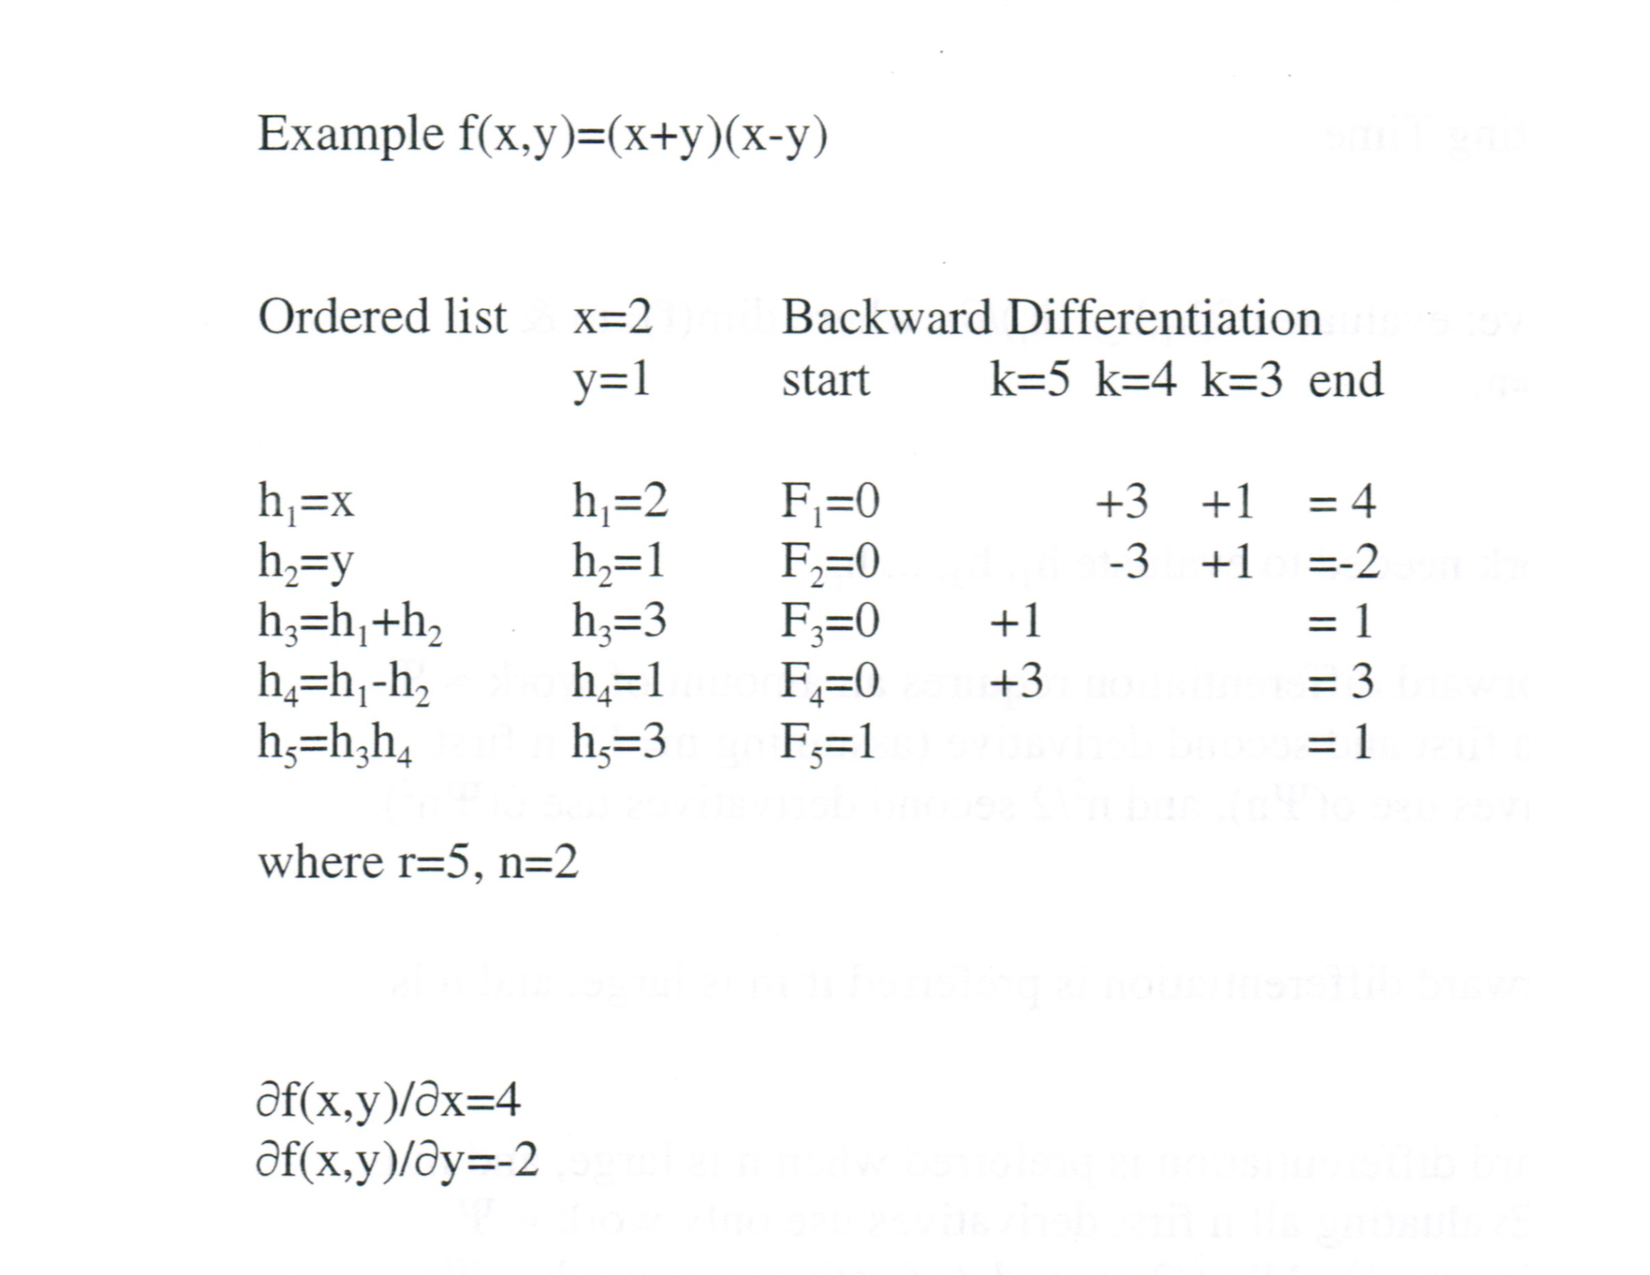
\includegraphics{BackwardsDifferentiationExample.pdf}}
   \caption{Example of Backwards Differentiation}
   \label{fig:BackwardsDifferentiation} 
\end{center}
\end{figure}

Second derivatives can be obtained by applying backwards differentiation twice, or by applying backwards differentiation and forwards differentiation in either order. Three work vectors each of length 
$r$ (the length of the list of recursions in the algorithm) are required. Let $\bf F$ be provided by the backwards differentiation algorithm above to compute all the derivatives of $h_r$. Let $\bf Q$ and $\bf S$ each be arrays also of length $r$. Then second derivatives can be computed using the following algorithm: 

\begin{align*}
1.~~ & \hbox{Initialize } Q_v = 1, Q_j = 0 \hbox{ and } v\in \{1,2,\hdots, n\} \hbox{ and } S_j = 0, \forall j = 1,2, \hdots, r\\
2.~~ & Q_k = Q_K + Q_i (\partial h_k/ \partial h_i), h \in \Omega_k; \\
        & S_j = S_j + Q_i F_k (\partial^2 h_k/\partial h_i \partial h_j), ~ h_i, h_k \in \Omega_k, ~ k = n+1, n+2, \hdots, r\\ 
3.~~ & S_j = S_j + S_k (\partial h_k/\partial h_i), ~h_j \in \Omega_k,~ k = r, r-1, \hdots, n+1\\
4.~~ & \hbox{Then } \partial^2 h_r/\partial x_v \partial x_j = S_i, ~ i = 1,2,\hdots,n\\
\end{align*}Note that $\bf Q$ is calculated by the forward differentiation equations and Step 3 is the first derivatives by backwards differentiation algorithm. This is an example of applying forwards differentation to the backwards differentiation algorithm in order to calculate the 2nd derivatives of $h_r$ with respect to the parameter set $\bf x$. As mentioned, one can also apply backwards differentation twice or forwards differentiation followed by backwards differentiation. The above keeps the bookkeeping aligned in the sense that all three work vectors $\bf F$, $\bf Q$ and $\bf S$ have the same length.


\section{Time Considerations}
Consider the case we we are evaluating a vector-valued function $\partial {\bf f}(h_1,h_2,\hdots,h_r)/\partial {\bf x}$ where $\hbox{dim}({\bf f}) = m$ and $\hbox{dim}({\bf x}) = n$. Let $\Psi$ equal the computational work need to evaluate $h_1, h_2, \hdots, h_r$.\\

Then forward differentiation requires and amount of computational work $\propto \Psi$ for each first and second derivative (assuming $m=1$): $n$ first derivatives use $o(n\Psi)$ and $n^2\Psi$ amount of 
work respectively. Nevertheless forward differentiation is preferred if $m$ is large and $n$ is small.\\

Backwards differentiation is preferred when $n$ is large and $m$ is small. Evaluating all $n$ first derivatives uses only work $\propto \Psi$ (assuming $m=1$). All $n^2/2$ second derivatives uses work 
$\propto n\Psi$.

%%%%  Example of Tabular Mode for Backwards Differentiaiton
%\vspace{0.25truein}
%First derivatives, $\partial F({\bf L}) / \partial x_v$, are summarized in the following table

%\begin{tabular}{l}
%Initializations:\\
%$\bf L$ is provided (see Table 1).\\
%{${\bf F}_{N \times N}$ is a work space with elements $F_{ij}$, defined respectively for $i \ge j$.}\\
%$\ominus_k =$ ``$+$'' if $k$-th diagonal is part of non-negative submatrix, ``$-$'' otherwise.\\
%$\pm_k = -\ominus_k$.\\
%$F_{ij} \leftarrow \partial F({\bf L})/\partial L_{ij}$\\
%\hline\\
%Algorithm:\\
%(a) ${\bf F} \leftarrow T({\bf F})$ by following operations:\\
%For $ k = N, ..., 1$ (N.B. Decreasing Order) do\\
%if $|L_{kk}| > \rm zero$, then do:\\
%$F_{ik} \leftarrow F_{ik} \pm_k (F_{ij} \times L_{jk})$, $F_{jk} \leftarrow F_{jk}  \pm_k (F_{ij} \times L_{ik})$, for  $j = k+1, ...,N$ \& $i = j, ..., N$\\
%$F_{jk} \leftarrow \ominus_k F_{jk}/L_{kk}$,  $F_{kk} \leftarrow F_{kk} \pm_k (F_{jk} \times L_{jk})$, for  $j = k+1, ...,N$\\
%$F_{kk} \leftarrow \ominus_k (1/2) F_{kk}/L_{kk}$\\
%end $k$\\
%\\
%\textcolor{red}{(b)   $\partial F({\bf L})/\partial x_v = \sum_{i \ge j} F_{ij}\times \partial K_{ij}/\partial x_v, \quad v = 1, 2, ... p.$}\\
%\\
%\hline\\
%Table 2. Pseudocode for Backward Differentiation of $F({\bf L})$.\\
%\end{tabular}
\section{Initialization of Orbit Determination}
The fitting methods described above require a good initial guess of the orbit and, because the prediction functions involved are non-linear in terms of the underlying parameters, proceed by iteration beginning with the initial guess. 

There are several classical orbit determination methods based on Angles-Only data: Laplace method of successive differentiation, Gauss's method, Escobal's Double-R Iteration method, etc. In the case of a single orbiting sensor there are severe limitations for short periods of observation due to the large number of completely different ballistic trajectories that match the Line-of-Sight data very closely. It is necessary to observe enough trajectory curvature in the orbit in order to single out the orbits which are good candidate initial states. Data from two orbiting sensors greatly improves initial state estimation.\\

Let us set up a time-dependent polynomial fit for the purposes of making a good initial state orbit estimation. The following represents a linear model for the $m$-vector polynomial 
$$Y(t) = X(t) \beta  + \epsilon.$$ The $m$-by-$n$+1 incidence matrix $X(t)$ is given by $$X(t) = [ \bf{I}~ |~ t \bf{I}~ |~ t^2 \bf{I}~|~ t^3 \bf{I}~|~ \hdots~ | t^n \bf{I} ] $$ and $I$ is the $m$-by-$m$ Identity matrix and $\epsilon$ is the uncertainty in the linear model. 

This method can be extended in a manner tailored for line of sight data and satisfy Newton's 2nd law. Because line of sight measurements are two dimensional the difference between the observed and predicted line of sight unit vectors needs to be projected into the perpendicular plane in order to compare with the estimated measurement error. Gravitation, at least up to $1/r^2$ contributions can be used as a constraint via Lagrange multipliers. In principal it is probably immaterial whether one minimizes the projected spatial vector difference or actually the projected unit-vector difference, since the minimums are closely related except for scaling and the purpose is just to estimate the initial state. As an example the spatial difference between the polynomial at time $t$ and the sensor measurement location $S$ and line of sight measured unit vector $\vec{u}$ is given by the difference between the polynomial and the closest position on the ray extending from the sensor towards the polynomial along the line of sight, i.e., $S - u^T(S-Y)$ or
$$\vec{r} = S - u^T(S-Y(t)) - Y(t) = (I - u^T)(S-Y(t))$$ and a $\chi^2$ can be constructed for this problem as follows

$$\chi^2 = \sum_{i=1}^N\, [S_i - Y(t_i)]^T [1-u_i^T]^T [I-u_i^T][S_i - Y(t_i)]  + \lambda^T[\ddot{Y(t_i)} + \mu {Y(t_i)\over |Y|^3}],$$

Since the line of sight data is 2-d the $[I-u^T]$ matrix can be replaced by a $3$-x-$2$ projection matrix that take 3-vectors and projects them into the plane perpendicular to the line of sight measurement. Both

$${\bf M}_{UV}(i) =
\begin{bmatrix}
\cos\theta_i\cos\phi_i & \cos\theta_i\sin\phi_i & -\sin\theta_i \\
-\sin\phi_i & \cos\phi_i & 0\\
\end{bmatrix}
$$

Now ${\bf M}_{UV}$ and $[I - u^T]$ are both rank-2 projection matrices which project spatial differences into the plane perpendicular to the line-of-sight direction and satisfy the following relationship: 
$${\bf M}_{UV} {\bf M}^T_{UV} = [I - u^T][I-u^T]^T$$Also the covariance matrix for the line-of-sight measurements are conformable with ${\bf M}_{UV}$ and we can insert them also into the objective function in place of $[I-u^T]$ as follows:
$$\tilde{\chi}^2 = \sum_{i=1}^N\, [S_i - Y(t_i)]^T {\bf M}^T_{UV}{\bf Cov}^{-1}_{UV} {\bf M}_{UV} [S_i - Y(t_i)]  + \lambda^T\big[\ddot{Y}(t_i) + \mu {Y(t_i)\over |Y|^3}\big],$$ which differs from the usual expression in that the displacements are not necessary with respect to unit vector line-of-sight displacements on the unit sphere. In practice that is somewhat immaterial to the minimization scheme and can always be put back in to calculate the fitted covariance of the $\beta$ parameters. 

We include here a description of Laplace's method of orbit determination which can be found in many books\cite{Bate} and papers \cite{Bell}. Laplace's technique requires a polynomial approximation to a sequence of $3-d$ vectors which can be obtained by using linear regression to fit the vector functional form using a linear model\cite{Rencher}.
$${\bf y}(t) = {\bf M(}t)\, {\bf \beta}$$where the {\it design matrix} ${\bf M}(t) = [{\bf X},{\bf X}t,{\bf X}t^2,\hdots,{\bf X}t^{n-1}]^T$ is the 3-by-3n unit matrix (in the case of 3-d vector polynomials ${\bf X}  = {\bf I}_3$ and $\bf \beta$ is a 3n-by-1 vector of {\it regression parameters}. The Least Squares estimate of the regression parameters given $i=1,2,\hdots, N$ data points is 
$$\hat{\beta} = \bigg[\sum_{i=1}^N\, {\bf M}^T(t_i) {\bf M}((t_i)\bigg]^{-1}\bigg[\sum_{i=1}^N\, {\bf M}^T(t_i) {\bf y}((t_i)\bigg]$$ The above method can be used to fit vector polynomials to sensor positions and line-of-sight vectors so that approximations can be made to the vector as well as its first and second derivatives with respect to time which are needed to apply Laplace's method.\\ 

Let us assume that we have at least three line-of-sight unit vector measured from the moving sensor (following the description in \cite{Bate})
\begin{align*}
{\bf L}_i = 
\begin{bmatrix}
L_I\\
L_J\\
L_K\\
\end{bmatrix}
= 
\begin{bmatrix}
\sin(\theta_i)\cos(\phi_i)\\
\sin(\theta_i)\sin(\phi_i)\\
\cos(\theta_i)\\
\end{bmatrix} = {\bf M_{UV}}(i) \quad i = 1,2,\hdots,N  \quad\hbox{assume $N\ge3$}
\end{align*}
Laplace's technique involves writing the slant range vector $\vec{\bf \rho} = \rho{\bf L}$ in terms of the line-of-site vector from the sensor to the target and then adding the sensor location with respect to the origin at the center of the earth $\bf R$ to obtain the vector location of the target with respect to the origin in the form
${\bf r} = \rho{\bf L} + {\bf R}$ and then using the polynomial fits to $\vec{L}$ and $\vec{R}$ and their derivatives to express the first and second derivatives of $\vec{r}$ in the form 
\begin{align*}
{\bf r} &= \rho{\bf L} + {\bf R}\\
\dot{\bf r} &= \dot\rho{\bf L} + \rho\dot{\bf L} + \dot{\bf R}\\
\ddot{\bf r} &= 2\dot\rho \dot{\bf L} + \ddot\rho{\bf L}+ \rho\ddot{\bf L} + \ddot{\bf R}\\
\end{align*}
At this point Laplace's method uses an approximation for $\ddot{\bf r}$ and Newton's 2nd Law to insert the $1/r^2$ approximate gravitational force law into the above system so that it can be written in the form of a linear system which can be used to set up an 8th order polynomial to solve for the distance of the target to the origin. After that equation is solved numerically, then the result can be back-substituted into the vector relationships to estimate the targets position and velocity at a particular time. That becomes the initial estimate for the least squares fitting method to use to start the iterations. This state vector can be transformed into Kepler classical elements or any other set of elements desired. 


%\section{Initial State Estimation}

There are several classical orbit determination methods based on Angles-Only data: Laplace method of successive differentiation, Gauss's method, Escobal's Double-R Iteration method, etc. In the case of a single orbiting sensor there are severe limitations for short periods of observation due to the large number of completely different ballistic trajectories that match the Line-of-Sight data equally well. It is necessary to observe enough trajectory curvature in the orbit in order to single out the orbits which are good candidate initial states. Data from two orbiting sensors greatly improves initial state estimation.\\

Let us set up a time-dependent polynomial fit for the purposes of making a good initial state orbit estimation. The following represents a linear model for the $m$-vector polynomial 
$$Y(t) = X(t) \beta  + \epsilon.$$ The $m$-by-$n$+1 incidence matrix $X(t)$ is given by $$X(t) = [ \bf{I}~ |~ t \bf{I}~ |~ t^2 \bf{I}~|~ t^3 \bf{I}~|~ \hdots~ | t^n \bf{I} ] $$ and $I$ is the $m$-by-$m$ Identity matrix and $\epsilon$ is the uncertainty in the linear model. 





\section{Line of Sight Displacements}
Using spherical polar coordinates we define a position on the unit sphere in terms of $\theta$ and $\phi$ as
$${\bf r} = [\sin\theta \cos\phi, ~\sin\theta \sin\phi, ~\cos\theta]$$We can define two tangent vectors to the unit sphere at $[\theta, \phi]$ by taking the derivative of the position vector with respect to the coordinates $\theta$ and $\phi$. Let $\bf u$ be the tangent vector in the $\theta$ direction and $\bf v$ be the tangent vector in the $\phi$ direction. 
By taking derivatives we have that these vectors are proportional to 
\begin{align*}
{\bf u} &\propto [\cos\theta \cos\phi, ~\cos\theta \sin\phi,~ -\sin\theta]\\
{\bf v} &\propto [-\sin\theta \sin\phi, ~\sin\theta \cos\phi, ~0]
\end{align*}
We will define $\bf u$ and $\bf v$ to be the respective unit vectors in the above directions: 
\begin{align*}
{\bf u} &=  [\cos\theta \cos\phi, ~\cos\theta \sin\phi, ~-\sin\theta]\\
{\bf v} &= [ -\sin\phi, ~\cos\phi, ~0]
\end{align*}
The three vectors $\{{\bf r}, {\bf u}, {\bf v} \}$ form an orthonormal set of vectors with $\bf r$ being along the line of sight and $\bf u$, $\bf v$ spanning directions in the plane perpendicular to the line of sight.
Coordinates in the perpendicular plane represent angular differences between two line of sight vectors and there are several ways of parameterizing these angular differences. For example we can project the vector differences between two line of sight vectors along $\bf u$ and $\bf v$ by taking dot products of those vector differences with these unit vectors. 
Alternatively we can take the dot product directly between the line of sight vectors and use polar coordinates where the radius represents the magnitude of the angular deflection. We can also use the angular differences $\Delta\theta$ and 
$\Delta\phi$, and we can work out expressions for the projections of the line of sight vectors in terms of their components using trigonometric identities. \\

Consider two line of sight vectors ${\bf l}_1$ and ${\bf l}_2$ and consider their vector difference in coordinate space:
$${\bf \Delta l} = {\bf l}_1 - {\bf l}_2$$ If we take the dot produce with the components perpendicular to, say ${\bf l}_1$ can be expressed as 
\begin{align*}
{\Delta u} &=  {\bf \Delta l} \cdot {\bf u} =  ~~{\Delta l}_x\cos\theta \cos\phi + {\Delta l}_y\cos\theta \sin\phi  -{\Delta l}_z\sin\theta\\
{\Delta v} &=  {\bf \Delta l} \cdot {\bf v} =  -{\Delta l}_x \sin\phi + {\Delta l}_y\cos\phi 
\end{align*} This set of relations can be cast in matrix form as
\begin{align*}
\begin{bmatrix}
\Delta u\\
\Delta v\\
\end{bmatrix} =
\begin{bmatrix}
\cos\theta \cos\phi & \cos\theta \sin\phi &-\sin\theta\\
-\sin\phi & \cos\phi & 0\\
\end{bmatrix}
\begin{bmatrix}
\Delta l_x\\
\Delta l_y\\
\Delta l_z\\
\end{bmatrix}\numberthis \label{eqnDeltaLOS}\end{align*}
which can be viewed as a transformation from a 3-dimensional space to a 2-dimensional space. The Jacobian of such a transformation has rank 2. 
Another way to express $[\Delta u, \Delta v]$ is in terms of the spherical polar coordinates of ${\bf l}_1$ and ${\bf l}_2$:
\begin{align*}
{\bf l}_1 &= [\sin\theta_1 \cos\phi_1, ~\sin\theta_1 \sin\phi_1, ~\cos\theta_1]\\
{\bf l}_2 &= [\sin\theta_2 \cos\phi_2, ~\sin\theta_2 \sin\phi_2, ~\cos\theta_2]
\end{align*}Let ${\bf l}_1$ define the line of sight direction and the coordinates $u, v$ will lie in the plane defined perpendicular to ${\bf l}_1$. Form the difference vector as 
$${\bf \Delta l} = 
\begin{bmatrix}
\sin\theta_1 \cos\phi_1 - \sin\theta_2 \cos\phi_2\\ 
\sin\theta_1 \sin\phi_1 - \sin\theta_2 \sin\phi_2 \\
\cos\theta_1 - \cos\theta_2\\
\end{bmatrix}
$$Taking the dot product with $\bf u$ and $\bf v$ defined in the perpendicular plane of ${\bf l}_1$ we have
\begin{align*}
\Delta u = {\bf \Delta l} \cdot {\bf u} &= (\sin\theta_1 \cos\phi_1 - \sin\theta_2 \cos\phi_2)\cos\theta_1\cos\phi_1\\
                                       &~~~+ (\sin\theta_1 \sin\phi_1 - \sin\theta_2 \sin\phi_2)\cos\theta_1 \sin\phi_1\\
                                       &~~~- (\cos\theta_1 - \cos\theta_2)\sin\theta_1\\ \\
\Delta v = {\bf \Delta l} \cdot {\bf v} &= -(\sin\theta_1 \cos\phi_1 - \sin\theta_2\cos\phi_2)\sin\phi_1\\
                                                      &~~~+ (\sin\theta_1 \sin\phi_1  - \sin\theta_2 \sin\phi_2)\cos\phi_1
\end{align*}
Using trigonometry the above relationship between $\Delta u$ and $\Delta v$ in terms of the angles defining the line of sight directions reduce to
\begin{align*}
{\Delta u} &=  \sin\theta_1\cos\theta_2 - \sin\theta_2\cos\theta_1\cos(\phi_1 - \phi_2)\\
{\Delta v} &=  \sin\theta_2\sin(\phi_1 - \phi_2)
\numberthis \label{eqnAngles}\end{align*}
Another representation that might be useful is to normalize the $[\Delta u, \Delta v]$ displacements so that each of the variables is bounded between $-1$ and $1$. As an example we could consider:
\begin{align*}
{\Delta \tilde u} &=  \sin\theta_1\cos\theta_2 - \sin\theta_2\cos\theta_1\cos(\phi_1 - \phi_2)\\
{\Delta \tilde v} &=  \sin(\phi_1 - \phi_2)
\numberthis \label{eqnNormalizeAngles}\end{align*}In this case the displacements lie in the rectangle $-1 \le \Delta \tilde u \le 1$ and $-1 \le \Delta \tilde v \le 1$. We have several representations Eq.\eqref{eqnDeltaLOS}, Eq.\eqref{eqnAngles}, and Eq.\eqref{eqnNormalizeAngles} with which to express the displacements in the perpendicular plane with respect to ${\bf l}_1$. The first relates the (x,y,z) components of the line of sight difference vector and a transformation Jacobian to arrive at $[\Delta u, \Delta v]$. The second relates the spherical polar angles of ${\bf l}_1$ and ${\bf l}_2$ to the differences $[\Delta u, \Delta v]$ as seen in the perpendicular plane and the third is a modified version of the second such that the possible displacements cover a fixed rectangular region.\\

The choice of which displacement representation to use depends on the details of the measurements and their covariance structure and how it fits in with the objective function, $\chi^2$, to be minimized in the orbit determination method.


\begin{thebibliography}{9}
\bibitem{Avery}{Paul Avery, ``Applied Fitting Theory I: Generalized Least Squares Theory, CBX-91-72''}
\bibitem{SQUAW}{O.I. Dahl, T.B. Day, F.T. Solmitz, N. L. Gould, ``Group A Programming Note No. P-126''}
\bibitem{Smith}{Stephen P. Smith, ``The Cholesky Decomposition and Its Derivatives''}
\bibitem{Escobal}{Escobal, ``Methods of Orbit Determination''}
\bibitem{B&C}{Brouwer and Clemence,`` Celestial Mechanics''}
\bibitem{Tapley}{Tapley, Schutz, Born, ``Statistical Orbit Determination''}
\bibitem{Griewank}{Griewank, {\it et al}\/., ``Computational Differentiation''}
\bibitem{JG&BK}{John Georganas, William Kovalcik, ``Angle Sensor Tracking Concepts''}
\bibitem{JG}{John Georganas, ``Converted Specific Angular Momentum Measurements Estimator''}
\bibitem{Keil}{Elizabeth M. Keil, ``Kalman Filter Implementation to Determing Orbit and Attitude of a Satellite in a Molniya Orbit''}
\bibitem{Bizup}{David R. Bizup, Donald E. Brown, ``The Over-Extended Kalman Filter -- Don't Use It!''}
\bibitem{Bate}{Roger R. Bate, Donald D. Mueller, Jerry E. White, ``Fundamentals of Astrodynamics'', Dover 1971, pp. 117-122}
\bibitem{Bell}{P.O. Bell, ``Orbit Determination by Angular Measurements''}
\bibitem{Claus}{A.J.Claus, R.B. Blackman, E.G. Halline, W.C. Riggway, III, ``Orbit Determination and Prediction and Computer Programs''}
\bibitem{Rencher}{Alvin C. Rencher and G. Bruce Schaalje, ``Linear Models in Statistics''}
 \end{thebibliography}
\end{document}
